\begin{spacing}{1.25}
\vskip 20pt
\noindent
\rule{0.49\textwidth}{0.75pt} $_{\Diamond}$ \rule{0.49\textwidth}{0.75pt}\\
{\Large{\textbf{Preface}}}\\
This chapter presents a study on non-contact stress assessment using the Deep Tabular Method. The aim is to evaluate stress levels using contactless techniques and  deep tabular methods.\\
\rule{0.49\textwidth}{0.75pt} $_{\Diamond}$ \rule{0.49\textwidth}{0.75pt}
\end{spacing}
\newpage





% \begin{figure}[ht]
% \centering
% 
\includegraphics[width=14cm]{Chapter2/Figures/CNN (2).png}	% height, width, scale, angle
% \caption{Convoutional Neural Network}
% \label{fig:arch}
% \end{figure}



\section{Introduction}\label{}
Stress is a physical, emotional, or mental response to external pressures or demands, which can arise from various 
 factors. Life situations like work challenges, family issues, and  environmental changes often arouse stress conditions in an individual. It is a natural response of the body to perceived threats and can manifest as tension, anxiety, or other psychological or physical reactions~\cite{giannakakis2019review}. Stress causes the body to release hormones like cortisol and adrenaline, which raise your heart rate, blood pressure, and blood sugar to help you deal with challenges. However, if stress lasts a long time, it can lead to serious health problems like heart disease, diabetes, anxiety, and depression~\cite{fink2010stress}.

In  human body autonomic nervous system (ANS) is responsible for controlling the number of heart-beats per minute~\cite{barazi2021dissecting}. ANS can be further divided into two sub-parts: (a) Sympathetic nervous system, 
  (b) Parasympathetic nervous system.
    Sympathetic  nervous system is active when an individual encounters situation like stress, anxiety, fear or undergoes laborious exercises, as a result it increases the heart rate. On the other hand parasympathetic nervous system is active when an individual is in calm state of mind particularly when an individual  feels compassion or love and thus, it decreases the heart-rate. As mentioned above heart rate is directly influenced by ANS which further depends upon our state-of-mind. Thus in this work we aim to estimate stress based on heart-rate (HR) and its related factors like  Heart rate variability (HRV), Peak detection etc.

    Traditionally, heart rate can be measured by various methods like electrocardiography (ECG), electromyography (EMG), and  photoplethysmography (PPG). However, these methods although accurate are cost-sensitive and requires direct physical contact. Henceforth, in this work we explore, non-invasive and cost insensitive method of heart-rate estimation by utilizing remote photoplethysmography (rPPG) signals.
rPPG extends traditional PPG by using camera technology and computer vision techniques to analyze visible light reflections on the skin. The reflected light detects blood volume changes caused by heartbeats  particularly from facial regions~\cite{speth2024mspm},\cite{mironenko2020remote}.

Over the years various computer vision and deep learning  based techniques have been reviewed to address challenges like motion artifacts and illumination variations in rPPG signals~\cite{lee2024review},\cite{wong2022optimising}. The method and color space selection greatly influence signal accuracy and reliability~\cite{zhao2024toward}. Techniques such as Plane-Orthogonal-to-Skin (POS)~\cite{lee2024review} are robust under varying lighting conditions, while Chrom-based methods~\cite{lee2024review} are more sensitive to skin color changes but  struggle with motion artifacts~\cite{pirzada2023remote}.

\begin{table*}[!h]
    \centering
    \caption{Comparative study of latest existing work}
    \begin{tabular}{p{3cm} p{4cm} p{2cm} p{5cm}} % Specify the width of each column
        \toprule
        \textbf{Author\& Year} & \textbf{Approach} & \textbf{Dataset} & \textbf{Remarks} \\ 
        \midrule
        Ziaratnia et al.(2024)\cite{ziaratnia2024multimodal} & Proposed framework based on combining Convolutional Transformer (CCT) and LSTM model. & UBFC-Phy & Large variation in reported results across different folds in case of multi-level stress classification.\\

        Xu et al.(2024)\cite{xu2024facial} & Proposed framework based on multi-task learning for stress detection.  & UBFC-Phy & Complex model architecture\\
        
        Pan et al.(2024)\cite{pan2024spatial} &Combines spatial and temporal attention modules to assign adaptive weights to features, utilizing a ResNet-style architecture to predict depression levels & AVEC2013, AVEC2014 & Data augmention is required for training the network. \\
        
        Casado et al.(2023)\cite{casado2023depression} & Pipeline methods to detect facial region and 60 statistical features are used to detect stress, utilizing random forest and multilayer perceptron networks & AVEC2013, AVEC2014 & Computation cost is high, supercomputer is used \\

        
        \bottomrule
    \end{tabular}
\end{table*}

Here, in this work for stress assessment, firstly rPPG signals are extracted from recorded video frames. Later, physiological features like HR, HRV etc are calculated from  observed rPPG signals. Further, the extracted physiological features are encoded for learning discriminative stress levels  by employing deep tabular data learning architecture~\cite{arik2021tabnet}  based on attention mechanism. Main  contributions of this work are as follows:
\begin{itemize}
    
    
    \item \textbf{Efficient Tabular Learning with TabNet:} The proposed method harnesses TabNet network ~\cite{arik2021tabnet} as the foundational backbone to directly process physiological features extracted from rPPG signals, incorporating built-in feature prioritization and sparsity mechanisms. This eliminates the need for extensive preprocessing while enhancing model interpretability and performance.
    
    \item \textbf{Improved Generalization Across Classification  Tasks:} The method demonstrates lower variance in accuracy across binary and multi-class stress classification tasks, highlighting superior generalization compared to existing approaches, which often exhibit significant performance variability.

    \item \textbf{Robust Feature Extraction:} To effectively manage the dynamic motion of faces across video frames and improve the precision of facial region extraction,the proposed method integrates the Haar Cascade~\cite{choi2022face}~\cite{hakim2019implementation} and Mediapipe library~\cite{lugaresi2019mediapipe}.This combination facilitates robust face detection and accurate localization of facial landmarks.
\end{itemize}

\begin{figure*}[!htp]
    \centering
    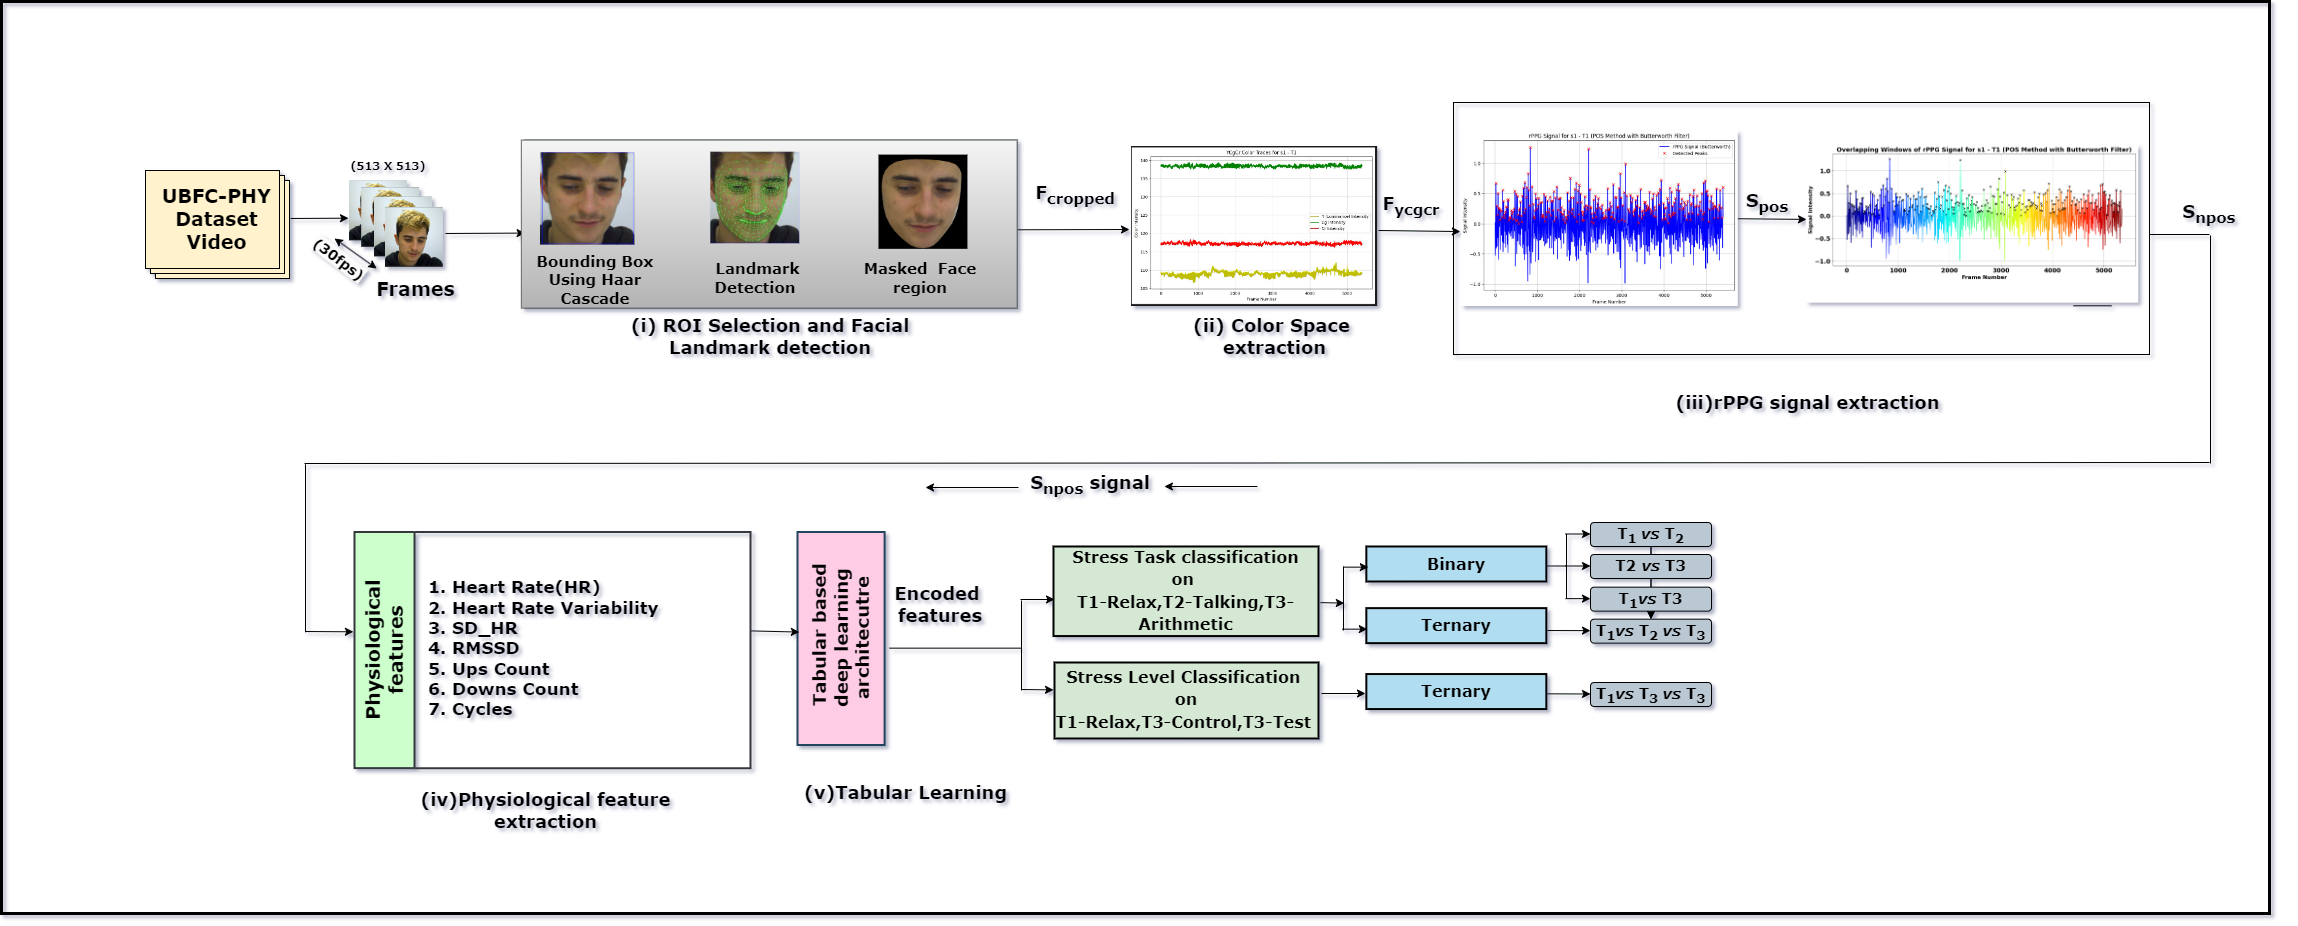
\includegraphics[width=\textwidth]{Chapter2/Figures/diagram (3).drawio.png}
    \caption{Proposed architecture comprising of five main parts: (i) ROI selection and facial landmark detection (ii) Color space  extraction (iii) rPPG signal extraction (iv) Physiological features extraction (v) Tabular learning on extracted physiological features}
    \label{fig:Encoder architecture}
\end{figure*}

The rest of this paper is organized as follows: Section 2 provides a brief description of the existing literature. Section 3 describes the proposed methodology in detail. In Section 4 description of the dataset is presented along with experimental results and analysis. Finally, Section 5 concludes this paper.

\section{Related Work}

Several works have been reported in the literature for rPPG signal analysis ~\cite{10155145}~\cite{speth2024mspm}~\cite{mcduff2023camera}  but the work done in the field of stress analysis using rPPPG signal is still limited. Table 1 lists some of the prominent work in stress detection using rPPG signals.


In one of the notable work ~\cite{ziaratnia2024multimodal} the author proposed a deep learning-based method utilizing Compact Convolutional Transformers (CCT) for feature extraction and Long Short-Term Memory (LSTM) for temporal pattern recognition. This study presents a non-contact approach to recognize stress using rPPG signals derived from RGB facial videos. In another work~\cite{xu2024facial}  a multi-task attentional convolutional neural network (MTASR) is deployed, which integrates peak detection and heart rate estimation to enhance stress recognition. Using peak detection as a physiological parameter, the researchers trained their network to identify more reliable physiological indicators. In another work, the authors
~\cite{casado2023depression} recognized depression based on a pipeline that extracts rPPG signals completely unsupervised and calculates $60$ statistical, geometrical and physiological features. These extracted features are used to train several machine learning regressors to recognize different levels of depression. In ~\cite{ntalampiras2023model}, the authors proposed a nonintrusive, low-cost, and automatic stress monitoring framework. This framework extracts multi-domain speech features to reveal complementary stress-related characteristics. The ensemble modeling provides a good solution to minimize computation time during  training.

In one of pioneer work in stress analysis domain
 authors  ~\cite{sloan1994effect}  proposed  an approach to analyzes $24$ hour electrocardiographic recordings of $33$ healthy subjects to examine how psychological stress affects cardiac autonomic control. This study focuses on Respiration rate (RR) interval, and heart period variability (HPV) analysis to evaluate the impact of stress.
In ~\cite{pan2024spatial} a deep  network for stress assessment  is proposed that focuses on facial features such as expressions, movements, and specific areas like the eyes, nasolabial folds, and jaw, which are related to depression. The proposed model emphasizes dynamic facial features through its attention mechanism.


\section{METHODOLOGY}

This section conceptualizes our proposed approach. Figure~\ref{fig:Encoder architecture} gives a generic overview of the proposed system which consists of mainly five parts: (i) ROI selection and facial landmark detection (ii) Color space extraction from cropped facial regions (iii) rPPG signal extraction (iv) Physiological features extraction from rPPG signals (v) Tabular learning on physiological features.

%The video data was converted into frames, with all videos processed at 30 frames per second (fps). This provided the individual frames for further analysis.

\subsection{ROI Selection and Facial Landmark Detection}
In the pre-processing phase, video frames are extracted from facial video sequences. Specifically, we utilize a frame rate of $30$ fps for temporal segmentation of the video. Each extracted frame is maintained at a resolution of $513 \times 513$ pixels. Following the frame extraction, the next step involves generating a bounding box around the facial region of interest. To achieve this, we implement the Haar Cascade algorithm~\cite{choi2022face}, which operates by detecting facial features through the application of rectangular filters that compute the intensity differences between adjacent regions in the image. Once the bounding box is delineated, the subsequent step is the detection of facial landmarks. For this, we employ the Mediapipe Face Mesh~\cite{lugaresi2019mediapipe} framework, which facilitates the identification of $478$ facial landmarks~\cite{ziaratnia2024multimodal}.

By integrating both techniques in our proposed method, we address the challenges inherent in extracting the facial region of interest. Figures~\ref{fig:sub_roi2} and~\ref{fig:sub_roi} demonstrate these challenges and highlight the improvements achieved through our approach.

Furthermore, convex hull based masking technique has been employed to isolate and emphasize the facial region. Mathematically, the convex hull is the smallest convex shape that can enclose all the points representing the facial landmarks. For this we have first created a binary mask with the same resolution as our extracted video frame resolution ($513 \times 513$). Formally, binary mask is described as:
\[
\text{mask}(x, y) = 
\begin{cases} 
255 & \text{if } (x, y) \text{ lies within the convex hull} \\
0 & \text{otherwise}
\end{cases}
\]
where \((x, y)\) denotes the pixel coordinates. The last step is to generate cropped facial region, which is generated as:
\[
\text{$F_{Cropped}$} = \text{$F_{Mediapipe}$} \land \text{mask}
\]
where, $F_{Mediapipe}$ is the output representing $478$ facial landmarks.
Here, the bitwise AND operation is used to retain only the pixel values of the facial region that fall within the convex hull, effectively setting all non-facial pixels to black. This selective masking technique highlights the facial features by suppressing irrelevant background elements.

\begin{figure}[!h]
    \centering
    % Subfigure a
    \subfigure[Without proper preprocessing]{
        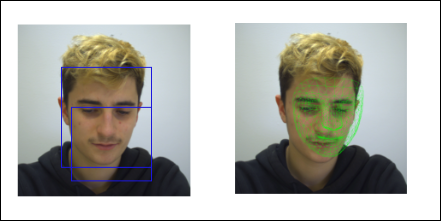
\includegraphics[width=0.45\textwidth, height=0.2\textheight]{Chapter2/Figures/ROI2.drawio.png}
        \label{fig:sub_roi2}
    }
    \hfill
    % Subfigure b
    \subfigure[After preprocessing]{
        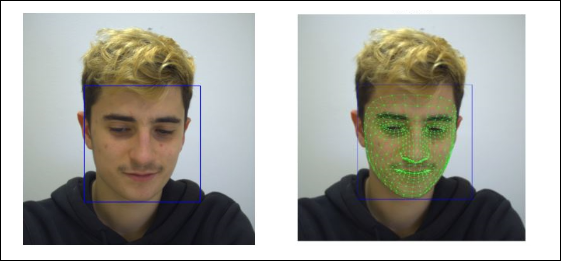
\includegraphics[width=0.45\textwidth, height=0.2\textheight]{Chapter2/Figures/ROI.drawio.png}
        \label{fig:sub_roi}
    }
    \caption{Preprocessing steps.}
    \label{fig:preprocessing_steps}
\end{figure}









\subsection{Color Space Extraction from cropped facial regions}
Inspired  by the prior study~\cite{kim2021non} we apply YCgCr color space ($F_{YCgCr}$) from  $F_{Cropped}$ (cropped facial region) as depicted in Figure~\ref{fig:color traces}.  By successfully decoupling the luminance component (Y) from the chrominance components (Cg) and (Cr), this color space facilitates the identification of subtle color changes that signify physiological conditions. By concentrating on the luminance channel and working with various skin tones, this color space lessens lighting variations~\cite{panigrahi2022non} ~\cite{ghazali2012innovative}.
\begin{figure}[h!]  % [h!] places the figure approximately here
    \centering
    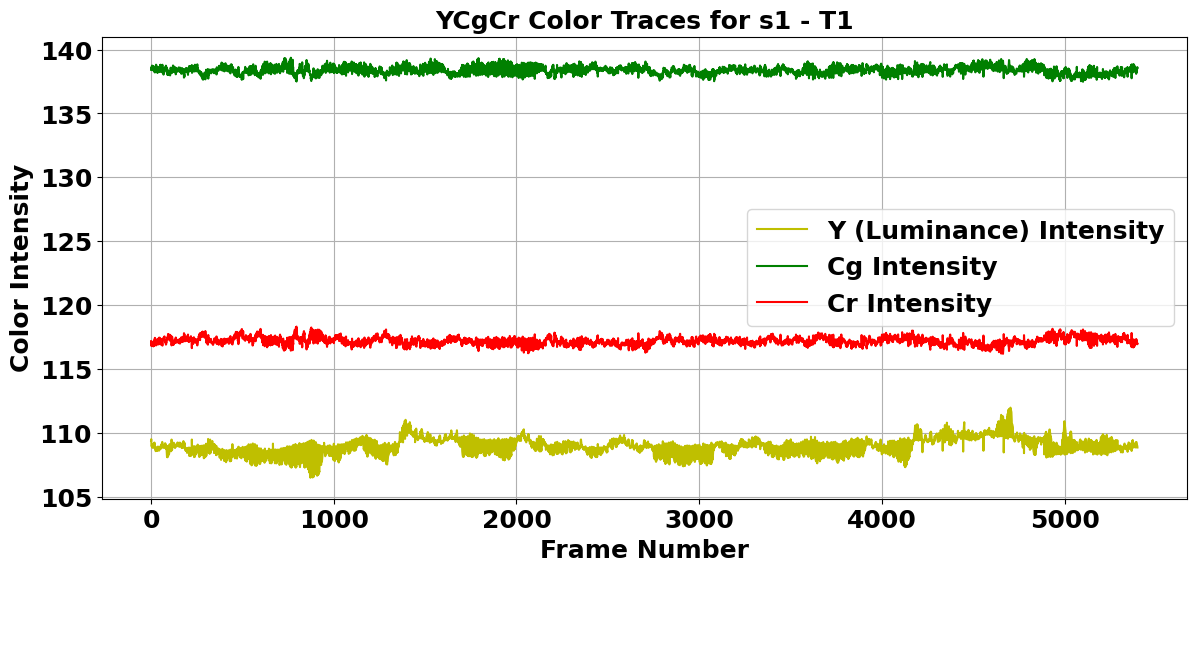
\includegraphics[width=0.8\textwidth, height=0.3\textheight]{Chapter2/Figures/color_trace.png}  % Adjust the width as needed
    \caption{YCgCr Color Traces}  % Caption for the image
    \label{fig:color traces}  % Label for referencing the image
\end{figure}

\subsection{rPPG Signal Extraction}
For extracting rPPG signals from $F_{\text{YCgCr}}$ we have utilized state-of-the-art POS (Plane-Orthogonal-to-Skin)~\cite{wang2016algorithmic} algorithm. Algorithm~\ref{alg:rppg} illustrates POS detailed steps.


\begin{algorithm}
\caption{ rPPG Signal Extraction}\label{alg:rppg}
\begin{algorithmic}[1]
    \State \textbf{Input:} $F_{\text{YCgCr}}$
    \State \textbf{Output:} $S_{\text{pos}}$ (extracted rPPG Signal)
    
    \State \textbf{Step 1: Compute Color Signals}
    \State $C_1 \gets Y - Cg$ \Comment{Color Signal 1}
    \State $C_2 \gets Cr - \frac{Y + Cg}{2}$ \Comment{Color Signal 2}
    
    \State \textbf{Step 2: Compute Means of Color Signals}
    \State $\mu_1 \gets \frac{1}{n} \sum_{i=1}^{n} C_{1i}$ \Comment{Mean of Color Signal 1}
    \State $\mu_2 \gets \frac{1}{n} \sum_{i=1}^{n} C_{2i}$ \Comment{Mean of Color Signal 2}
    
    \State \textbf{Step 3: Adjust Color Signals by Subtracting the Mean}
    \State $S_1 \gets C_1 - \mu_1$ \Comment{Adjusted Signal 1}
    \State $S_2 \gets C_2 - \mu_2$ \Comment{Adjusted Signal 2}
    
    \State \textbf{Step 4: Compute Final rPPG Signal}
    \State $S_{\text{pos}} \gets S_1 + S_2$ \Comment{rPPG Signal}
    
    \State \textbf{Return} $S_{\text{pos}}$
\end{algorithmic}
\end{algorithm}
Inspired by the prior study~\cite{xu2024facial} to normalize extracted rPPG signals ($S_{\text{pos}}$) we have filtered it with Butterworth filter~\cite{selesnick1998generalized}. While filtering  low cut-off frequency was set as $0.7$ Hz and  high cut-off frequency was set as  $2.5$ Hz.  Once the signals are normalized, we divide them into $2$-second windows ($30$ frames per second) with a $10\%$ overlap between segments to account for temporal differences across frames.

\begin{figure}[]  % [h!] places the figure approximately here
    \centering
    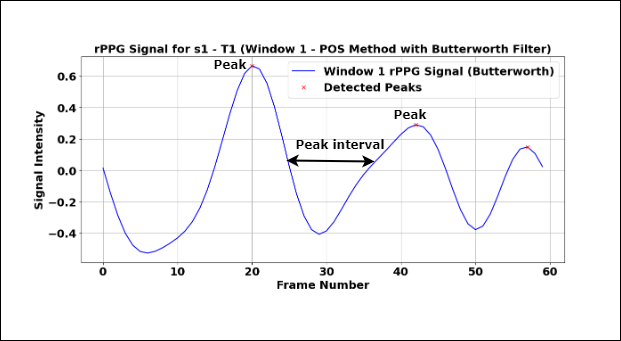
\includegraphics[width=0.8\textwidth, height=0.3\textheight]{Chapter2/Figures/window_peak.drawio.png}  % Adjust the width as needed
    \caption{Single window depicting signal peak and interval detection.}  % Caption for the image
    \label{fig:peak}  % Label for referencing the image
\end{figure}


\begin{figure*}[!htp]
    \centering
    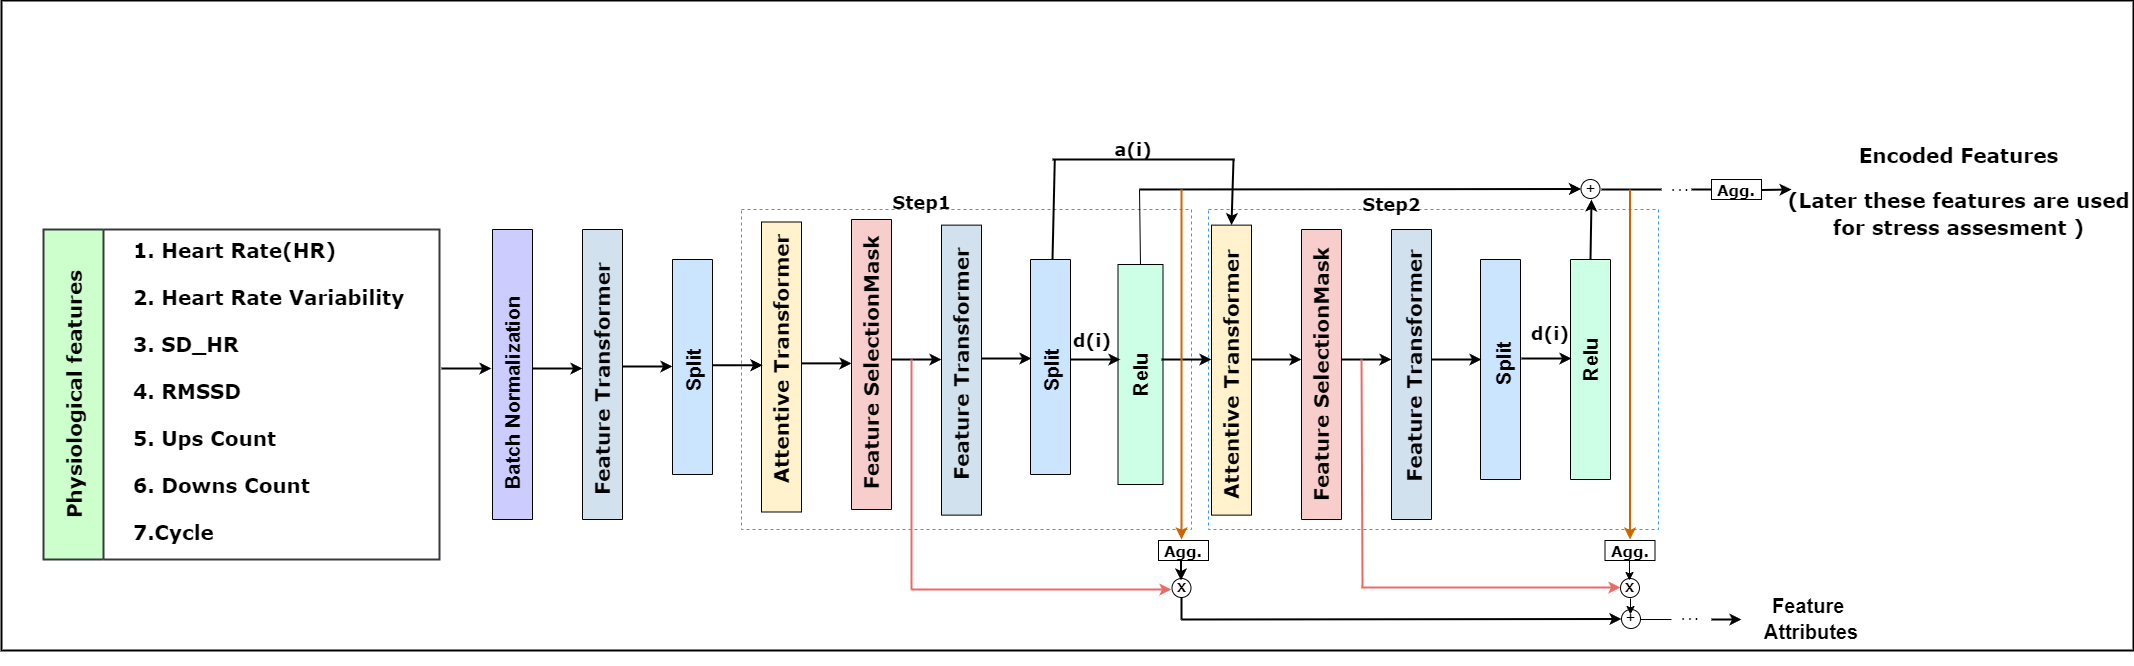
\includegraphics[width=\textwidth]{Chapter2/Figures/cnn_architecture (1).drawio.png}
    \caption{Encoder architecture for extracting discriminative information from physiological features. This architecture operates through a series of sequential decision steps mainly comprising of three parts (i) Feature Transformer (ii) Attentive Transformer (iii) Feature Selection Mask. Here,  \(a[i]\) serves as the input for the attention transformer in the next decision step while \(d[i]\), denotes the current decision output. }
    \label{fig:CNN architecture}
\end{figure*}



\subsection{Physiological Features Extraction}
From the normalized rPPG signals ($S_{\text{npos}}$) we have extracted signal peaks as shown in Figure~\ref{fig:peak}. From the extracted peaks, signal peak  intervals are computed as depicted in Figure~\ref{fig:peak}. Later on the basis of aforementioned signal intervals $7$ physiological features are computed as follows:



\begin{enumerate}
\item 
\textbf{Heart Rate (HR):}
\[
HR = \frac{60}{\text{mean interval between peaks (seconds)}}
\]
where intervals are the time differences between consecutive $S_{\text{npos}}$ peaks.

\item 
\textbf{Heart Rate Variability (HRV):}
\[
HRV = \text{Standard deviation of intervals (seconds)}
\]
which represents the variation in time between heartbeats.

\item 
\textbf{Standard Deviation of Heart Rate (SD\_HR):}
\[
SD\_HR = \text{Standard deviation of computed heart rates 
}
\]
(bpm) calculated for each interval.

\item 
\textbf{Root Mean Square of Successive Differences (RMSSD):}
\[
RMSSD = \sqrt{\frac{1}{N-1} \sum_{i=1}^{N-1} (\text{interval}_{i+1} - \text{interval}_i)^2}
\]
where \( N \) is the number of intervals, indicating short-term HRV.

\item 
\textbf{Ups Count}: In a sympathetic activity in Autonomic nervous system(ANS) this ups count refer to the number of times  $S_{\text{npos}}$ signal transit from a lower value to higher value. It indicates the onset of a heartbeat.

\item 
\textbf{Downs Count}: It is the moment when the heart finishes pumping blood and start to relax, which is captured as a downward transition in the $S_{\text{npos}}$ signal.

\item 
\textbf{Cycles}: Mathematically it is defined as the minimum of Ups Count and Downs Count.

\end{enumerate}





\subsection{Tabular Learning on Physiological Features}

The extracted physiological features are numeric values; thus, we store them in a tabular structure. To extract meaningful information from it, we have incorporated the state-of-the-art tabular learning architecture, TabNet~\cite{arik2021tabnet}. In our proposed methodology, we have extracted discriminative information from physiological features by utilizing the TabNet encoder architecture, as depicted in Figure~\ref{fig:CNN architecture}. This tabular-based deep learning architecture operates through a series of sequential decision steps, where each step refines its focus based on the information processed from the previous step. Each decision step employs non-linear transformations to refine the feature representations. Furthermore, it includes a sparsity regularization mechanism to control the number of features selected at each step. 

As depicted in Figure~\ref{fig:CNN architecture}, this architecture mainly comprises three modules: (i) Feature Transformer, (ii) Attentive Transformer, and (iii) Feature Selection Mask. All these are described below:

\textbf{Feature Transformer:} This module is responsible for transforming the input physiological features into meaningful representations. These representations are later divided into two parts using a split block. The first part, denoted as \(d[i]\) (as depicted in Figure~\ref{fig:CNN architecture}), contributes to the current decision output, while the other part, denoted as \(a[i]\) (as depicted in Figure~\ref{fig:CNN architecture}), serves as the input for the attentive transformer in the next decision step.

\textbf{Attentive Transformer:} This module generates a trainable mask that identifies the most important features for each decision step using a sparsemax function, which creates a sparse, interpretable feature selection mechanism. A prior scale term is also employed to regulate how often each feature is selected across decision steps.

\textbf{Feature Selection Mask:} This module is used for selecting globally important feature attributions.

To develop a deep tabular learning model capable of robustly identifying and prioritizing specific features derived from rPPG signals that play a critical role in our analysis, we leverage the TabNet architecture. This approach eliminates the need for preprocessing techniques by allowing the model to adaptively focus on essential features. If a feature is deemed less supportive at any stage, the model advances to another level of evaluation to reassess its importance.


\section{Experiment and Results} This section gives details about the experimental settings such as data-set, evaluation metrics, results along with training and testing protocol.

\subsection{Dataset Description} To validate the performance of proposed approach  in this work we have worked on UBFC-Phy dataset~\cite{sabour2021ubfc}. This dataset is publicly available and consists of $56$ subjects in total. Out of these $56$ subjects $47$ subjects are female and rest are male. This dataset contains facial videos of enrolled subjects. Each subject underwent  three different tasks: resting task (T1), speech task (T2) and arithmetic task (T3) resulting in generation of $168$ videos in total. Furthermore, this dataset is divided into two groups based on the challenging nature of the task namely: control group and test group. In control group subjects faced less challenging task as compared to subjects in test group.
\subsection{Model Validation and Experimental Setup } \label{validate}
For validating our proposed approach we have conducted two set of experimentation as conducted in previous state of the art work~\cite{ziaratnia2024multimodal} namely:
\begin{enumerate}
\item Stress task classification
\item Multi-level stress classification
\end{enumerate}
In stress task classification subjects are classified on the basis of tasks performed. Under this we have performed both binary ($T1$ vs. $T2$, $T2$ vs. $T3$, and $T1$ vs. $T3$) as well as ternary classification ($T1$ vs. $T2$ vs. $T3$). While in case of multi-level stress classification subjects are classified on the basis of the challenging nature of the task. Out of the three tasks $T3$ (arithmetic task)  is considered as the most demanding task~\cite{ziaratnia2024multimodal}. Thus, this set of experimentation is focused towards  classifying stress into three levels: (i) no stress ( $T1$ task for both control and test group), (ii) low stress ( $T3$ control group), and (iii) high stress ( $T3$ test group). For stress task classification seven-fold cross-validation technique and for multi-level stress classification stratified five-fold cross-validation technique has been adopted as in~\cite{ziaratnia2024multimodal}.The model was trained for 300 epochs for both sets of experiments.

All the experiments have  been conducted on a system with specifications as: Intel(R) Xeon(R) Silver 4114 CPU, 64 GB of RAM,  4 TB SSD,  NVIDIA GeForce GTX 1080 Ti GPU. For the software environment, we  have utilized  libraries such as 
 OpenCV ~\cite{mordvintsev2017opencv}, Python~\cite{de2012pattern}, PyTorch~\cite{imambi2021pytorch}, and Mediapipie~\cite{lugaresi2019mediapipe}.


\subsection{Performance Metrics}
The proposed framework is evaluated using common classification criteria such as accuracy, precision, recall, and F1 score.


\textbf{Accuracy:}
 Accuracy is calculated as the ratio of correctly predicted instances to total instances:

\[
\text{Accuracy} = \frac{TP + TN}{TP + FP + TN + FN}
\]
where:


True Positives (correctly predicted positive cases) and True Negatives (correctly predicted negative cases) are represented by the terms $TP$ and $TN$, respectively. False Positives (positive cases that were incorrectly predicted) and False Negatives (negative instances that were incorrectly predicted) are represented by the terms $FP$ and $FN$, respectively.
%\begin{itemize}
 %   \item $TP$ = True Positives (instances correctly classified as positive)
  %  \item $TN$ = True Negatives (instances correctly predicted negative )
   % \item $FP$ = False Positives (instances incorrectly predicted positive )
    %\item $FN$ = False Negatives (instances incorrectly predicted negative )
%\end{itemize}



\textbf{Precision:}Precision is the ratio of accurately predicted positive cases to all instances predicted as positive:

\[
\text{Precision} = \frac{{TP}}{{TP} +{FP}}
\]

\textbf{Recall:}Recall is the proportion of accurately predicted positive instances relative to all actual positive instances, including those incorrectly classified as negative. 
\[
\text{Recall} = \frac{TP}{TP + FN}
\]

\textbf{F1 Score:} It is calculated as the 
  harmonic mean of precision and recall. It is expressed mathematically as:
\[
F1 = 2 \cdot \frac{\text{Precision} \cdot \text{Recall}}{\text{Precision} + \text{Recall}}
\]
\subsection{Stress Task Classification Performance} As mentioned in section~\ref{validate} for stress task classification experimentation we have computed results for both binary as well as ternary classification.
Table~\ref{binary_1}, Table~\ref{binary_2}, and Table~\ref{binary_3} illustrates  binary stress classification results for T1 (resting task) vs. T2 (speech task), T1 (resting task) vs. T3 (arithmetic task), and T2 (speech task) vs. T3 (arithmetic task) tasks respectively. Table~\ref{ternary} illustrates ternary stress task classification results for  T1 (resting task) vs. T2 (speech task) vs. T3 (arithmetic task). Major observations from  Table~\ref{binary_1}, Table~\ref{binary_2}, Table~\ref{binary_3}, and Table~\ref{ternary} are as follows:
\begin {itemize}
\item  Highest accuracy is observed while differentiating subjects undergoing resting task versus  arithmetic task as depicted in Table~\ref{binary_2}. As stated in ~\cite{ziaratnia2024multimodal} arithmetic task is the most challenging task  and our proposed approach effectively discriminates it which depicts our model superiority.
\item Lowest  recall  is observed while differentiating subjects undergoing speech task versus  arithmetic task as depicted in Table~\ref{binary_3}. This phenomenon is quite obvious because speech task that involves expressing views in front of others and solving arithmetic problems both involved inducing stress in individuals.
\item  In case  of ternary stress task classification task as depicted in Table~\ref{ternary} the mean accuracy, precision  and recall across 7-folds are almost same. This phenomenon indicates fairness of our model which  focuses not only  on minimizing false negatives but also focuses on minimizing false positives.
\end {itemize}
\begin{table}[ht]
\centering
\caption{Stress task 7-fold cross-validation classification results. Binary classification \textbf{T1 (resting task) vs. T2 (speech task)}}
\label{binary_1}
\resizebox{0.70\textwidth}{!}{ % You can adjust the width and height here
    \begin{tabular}{|c|c|c|c|c|}
    \hline
    \textbf{K-folds} & \textbf{Accuracy} & \textbf{Precision} & \textbf{Recall} & \textbf{F1 score} \\ \hline
    Fold-1 & 0.750 & 0.833 & 0.625 & 0.714 \\ \hline
    Fold-2 & 0.681 & 0.615 & 1.000 & 0.761 \\ \hline
    Fold-3 & 0.812 & 0.727 & 1.000 & 0.842 \\ \hline
    Fold-4 & 1.000 & 1.000 & 1.000 & 1.000 \\ \hline
    Fold-5 & 0.937 & 0.888 & 1.000 & 0.941 \\ \hline
    Fold-6 & 0.937 & 0.888 & 1.000 & 0.941 \\ \hline
    Fold-7 & 0.875 & 1.000 & 0.750 & 0.857 \\ \hline
    \textbf{7-Fold Mean} & \textbf{0.857} & \textbf{0.850} & \textbf{0.9107} & \textbf{0.865} \\ \hline
    \end{tabular}
}

\end{table}

\begin{table}[ht]
\centering
\caption{Stress task 7-fold cross-validation classification results. Binary classification \textbf{T1 (resting task) vs. T3 (arithmetic task)}}
\label{binary_2}
\resizebox{0.70\textwidth}{!}{ % You can adjust the width and height here
    \begin{tabular}{|c|c|c|c|c|}
    \hline
    \textbf{K-folds} & \textbf{Accuracy} & \textbf{Precision} & \textbf{Recall} & \textbf{F1 score} \\ \hline
    Fold-1 & 0.812 & 0.857 & 0.750 & 0.800 \\ \hline
    Fold-2 & 1.000 & 1.000 & 1.000 & 1.000 \\ \hline
    Fold-3 & 0.937 & 1.000 & 0.875 & 0.933 \\ \hline
    Fold-4 & 0.930 & 1.000 & 0.875 & 0.933 \\ \hline
    Fold-5 & 1.000 & 1.000 & 1.000 & 1.000 \\ \hline
    Fold-6 & 1.000 & 1.000 & 1.000 & 1.000 \\ \hline
    Fold-7 & 0.937 & 0.888 & 1.000 & 0.941 \\ \hline
    \textbf{7-Fold Mean} & \textbf{0.946} & \textbf{0.963} & \textbf{0.928} & \textbf{0.944} \\ \hline
    \end{tabular}
}

\end{table}

\begin{table}[ht]
\centering
\caption{Stress task 7-fold cross-validation classification results. Binary classification \textbf{T2 (speech task) vs. T3 (arithmetic task)}}
\label{binary_3}
\resizebox{0.70\textwidth}{!}{ % You can adjust the width and height here
    \begin{tabular}{|c|c|c|c|c|}
    \hline
    \textbf{K-folds} & \textbf{Accuracy} & \textbf{Precision} & \textbf{Recall} & \textbf{F1 score} \\ \hline
    Fold-1 & 0.750 & 0.833 & 0.625 & 0.714 \\ \hline
    Fold-2 & 0.875 & 0.875 & 0.875 & 0.875 \\ \hline
    Fold-3 & 0.812 & 0.857 & 0.750 & 0.800 \\ \hline
    Fold-4 & 0.875 & 1.000 & 0.750 & 0.857 \\ \hline
    Fold-5 & 0.812 & 0.857 & 0.750 & 0.800 \\ \hline
    Fold-6 & 0.875 & 1.000 & 0.750 & 0.857\\ \hline
    Fold-7 & 0.937 & 0.888 & 1.000 & 0.941 \\ \hline
    \textbf{7-Fold Mean} & \textbf{0.848} & \textbf{0.901} & \textbf{0.785} & \textbf{0.835} \\ \hline
    \end{tabular}
}

\end{table}

\begin{table}[ht]
\centering
\caption{ Stress task 7-fold cross-validation classification results. Ternary classification \textbf{ T1 (resting task) vs. T2 (speech task) vs. T3 (arithmetic task)} }
\label{ternary}
\resizebox{0.70\textwidth}{!}{ % You can adjust the width and height here
    \begin{tabular}{|c|c|c|c|c|}
    \hline
    \textbf{K-folds} & \textbf{Accuracy} & \textbf{Precision} & \textbf{Recall} & \textbf{F1 score} \\ \hline
    Fold-1 & 0.750 & 0.757 & 0.750 & 0.752 \\ \hline
    Fold-2 & 0.750 & 0.795 & 0.750 & 0.752 \\ \hline
    Fold-3 & 0.875 & 0.891 & 0.875 & 0.873 \\ \hline
    Fold-4 & 0.916 & 0.933 & 0.916 & 0.918 \\ \hline
    Fold-5 & 0.833 & 0.838 & 0.833 & 0.829 \\ \hline
    Fold-6 & 0.916 & 0.933 & 0.916 & 0.918\\ \hline
    Fold-7 & 0.916 & 0.933 & 0.916 & 0.918 \\ \hline
    \textbf{7-Fold Mean} & \textbf{0.851} & \textbf{0.869} & \textbf{0.851} & \textbf{0.851} \\ \hline
    \end{tabular}
}

\end{table}
\subsection{Multi-Level Stress Classification Performance} Table~\ref{tab:stress_level_classification} and Table~\ref{stress_level_2} depicts results for multi-level stress classification. According to state-of-the-art research, we employed a 5-fold stratified cross validation strategy in this experiment because the number of subjects in the control and test groups was unbalanced~\cite{ziaratnia2024multimodal}. As depicted in Table~\ref{tab:stress_level_classification} the highest accuracy reported across all folds was in fold-4 while the mean accuracy achieved was $87.5\%$. Furthermore, as depicted in Table~\ref{stress_level_2}  the highest and lowest  multi-level stress accuracy was achieved in No-Stress and High-Stress class respectively.

\begin{table}[ht]
\centering
\caption{ Multi-Level stress 5-fold cross-validation classification results. Ternary classification: \textbf { no stress (T1 task for both control and test group), low stress (T3 control group) and high stress (T3 test group).}}
\label{tab:stress_level_classification}
\resizebox{0.70\textwidth}{!}{ % You can adjust the width and height here
    \begin{tabular}{|c|c|c|c|c|}
    \hline
    \textbf{K-folds} & \textbf{Accuracy} & \textbf{Precision} & \textbf{Recall} & \textbf{F1 score} \\ \hline
    Fold-1 & 0.826 & 0.896 & 0.826 & 0.816 \\ \hline
    Fold-2 & 0.869 & 0.864 & 0.869 & 0.864 \\ \hline
    Fold-3 & 0.863 & 0.877 & 0.863 & 0.857 \\ \hline
    Fold-4 & 0.954 & 0.961 & 0.954 & 0.953 \\ \hline
    Fold-5 & 0.863 & 0.865 & 0.863 & 0.861 \\ \hline
    \textbf{5-Fold Mean} & \textbf{0.875} & \textbf{0.882} & \textbf{0.875} & \textbf{0.870} \\ \hline
    \end{tabular}
}

\end{table}
\begin{table}[htbp]
\centering
\caption{ Multi-Level stress 5-fold cross-validation classification results. Mean value ($\pm$ standard deviations)  for three class classification individually:
\textbf { no stress (T1 task for both control and test group), low stress (T3 control group) and high stress (T3 test group) .}}
\label{stress_level_2}
\resizebox{0.80\textwidth}{!}{ % You can adjust the width and height here
    \begin{tabular}{|c|c|c|c|c|}
    \hline
    \textbf{Class} & \textbf{Accuracy} & \textbf{Precision} & \textbf{Recall} & \textbf{F1 score} \\ \hline
    No Stress & 0.981($\pm$0.040) & 0.910($\pm$0.092) & 0.981($\pm$0.040) & 0.943($\pm$0.061) \\ \hline
    Low Stress & 0.866($\pm$0.139) & 0.812($\pm$0.059) & 0.866($\pm$0.139) & 0.835($\pm$0.088) \\ \hline
     High Stress & 0.653($\pm$0.086) & 0.910($\pm$0.124) & 0.653($\pm$0.086) & 0.756($\pm$0.081) \\ \hline
    \end{tabular}
}

\end{table}
\begin{table*}[btp]
    \centering
    \caption{Experimental results comparing our approach to other cutting-edge techniques for stress task categorisation on the UBFC-Phys dataset. The best findings are bolded in the table, which displays the mean values (± standard deviations) of the $7$ cross-validation. This table's values are derived from ~\cite{ziaratnia2024multimodal}.}
    \label{compare_1}
    \resizebox{0.90\textwidth}{!}{ % This will resize the table to fit within the page
    \begin{tabular}{lcccccc}
        \toprule
        \textbf{Methods} & \multicolumn{2}{c}{\textbf{T1 vs. T2}} & \multicolumn{2}{c}{\textbf{T1 vs. T3}} & \multicolumn{2}{c}{\textbf{T1 vs. T2 vs. T3}} \\
        & \textbf{Accuracy} & \textbf{F1 Score} & \textbf{Accuracy} & \textbf{F1 Score} & \textbf{Accuracy} & \textbf{F1 Score} \\
        \midrule
        MLP~\cite{dolmans2021perceived} & 0.709(±0.061) & 0.706(±0.064) & 0.599(±0.040) & 0.587(±0.037) & 0.440(±0.028) & 0.434(±0.031) \\
        LIT~\cite{dolmans2021perceived} & 0.701(±0.063) & 0.699(±0.066) & 0.625(±0.042) & 0.622(±0.052) & 0.447(±0.027) & 0.443(±0.031) \\
        DFAF~\cite{gao2019dynamic} & 0.758(±0.035) & 0.756(±0.033) & 0.689(±0.040) & 0.686(±0.037) & 0.478(±0.034) & 0.477(±0.036) \\
        CAM~\cite{praveen2021cross} & 0.726(±0.060) & 0.722(±0.063) & 0.650(±0.052) & 0.645(±0.054) & 0.494(±0.028) & 0.487(±0.033) \\
        MFN~\cite{yu2021modality} & 0.769(±0.035) & 0.763(±0.043) & 0.684(±0.050) & 0.670(±0.049) & 0.501(±0.038) & 0.500(±0.036) \\
        BCSA~\cite{zhang2023dynamic} & 0.818(±0.063) & 0.817(±0.063) & 0.723(±0.039) & 0.722(±0.039) & 0.558(±0.052) & 0.552(±0.048) \\
        Multimodal CCT-LSTM~\cite{ziaratnia2024multimodal}  & \textbf{0.981(±0.016)} & \textbf{0.981(±0.016)} & 0.924(±0.037) & 0.924(±0.037) & 0.832(±0.058) & 0.834(±0.056) \\
       Proposed Approach & 0.857(±0.104) & 0.865(±0.095) & \textbf{0.946(±0.062)} & \textbf{0.943(±0.065)} & \textbf{0.851(±0.069)} & \textbf{0.851(±0.070)} \\
        \bottomrule
    \end{tabular}
    }
    
\end{table*}
\begin{table}[htbp]
\centering
\caption{Experimental findings comparing our proposed approach with state-of-the-art technique for multi-level stress classification using the UBFC-Phys dataset. The best findings are bolded in the table, which displays the mean values (± standard deviations) of the $5$-fold stratified cross-validation.}
\label{compare_2}
\small % Adjust the font size to make the table content more compact
\resizebox{0.80\textwidth}{!}{ % Adjust the table width to fit the page more appropriately
    \begin{tabular}{@{}l c c@{}} % Adjusting column spacing to make the table more compact
        \toprule
        \textbf{Methods} & \multicolumn{2}{c}{\textbf{T1 vs T3(ctrl) vs T3(Test) }} \\ % New header spanning two columns
        \cmidrule(lr){2-3} % Line under the merged header
        & \textbf{Accuracy} & \textbf{F1 Score} \\
        \midrule
        Multimodal CCT-LSTM~\cite{ziaratnia2024multimodal} & 0.805(±0.094) & 0.803(±0.095) \\ 
        Proposed Approach & \textbf{0.875(±0.047)} & \textbf{0.870(±0.050)}\\
        \bottomrule
    \end{tabular}
}
\end{table}

\begin{figure*}[!h]
    \centering

    \subfigure[]{
        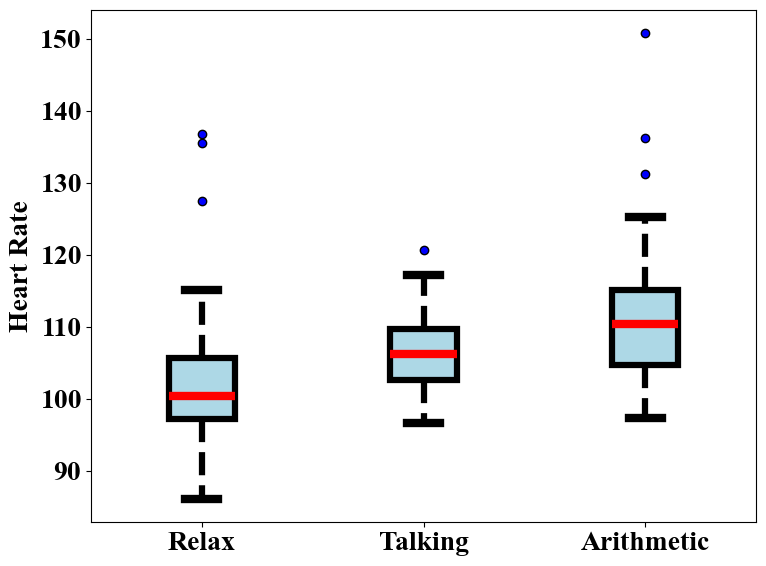
\includegraphics[width=0.45\textwidth]{Chapter2/Figures/HR.png}
        \label{fig:subfig1}
    }
    \hspace{0.02\textwidth}
    \subfigure[]{
        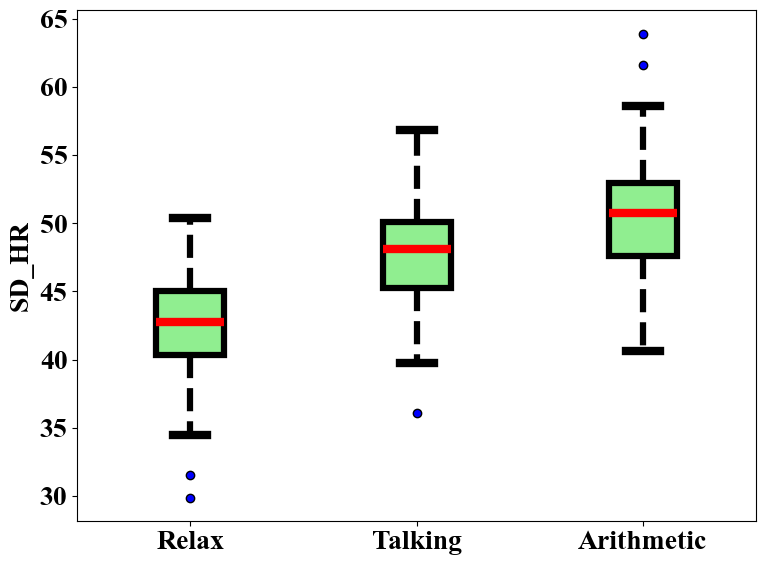
\includegraphics[width=0.45\textwidth]{Chapter2/Figures/SD_HR.png}
        \label{fig:subfig2}
    }
    
    \vspace{1em} % Add vertical spacing between rows if needed

    \subfigure[]{
        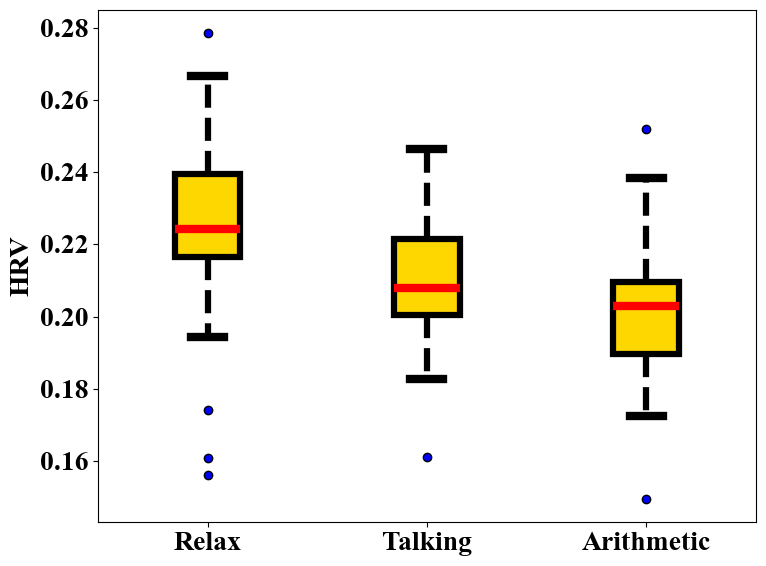
\includegraphics[width=0.45\textwidth]{Chapter2/Figures/HRV.png}
        \label{fig:subfig3}
    }
    \hspace{0.02\textwidth}
    \subfigure[]{
        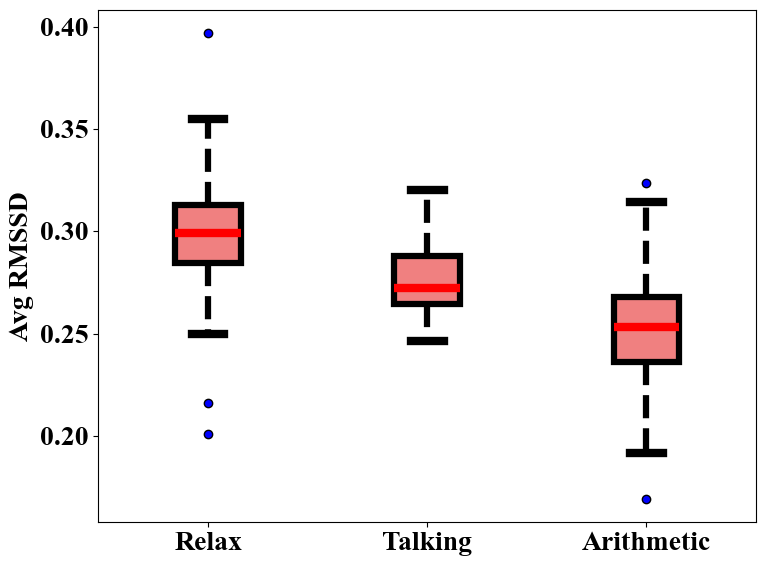
\includegraphics[width=0.45\textwidth]{Chapter2/Figures/Avg_RMMSD.png}
        \label{fig:subfig4}
    }

    \caption{Box Plots of $4$ physiological features: (a) Heart Rate (HR), (b) Standard Deviation of Heart Rate ($SD\_HR$), (c) Heart Rate Variability (HRV), and (d) Root Mean Square of Successive Differences (RMSSD).}
    \label{fig:mainfigure}
\end{figure*}



\subsection{Comparative Analysis} To validate the efficacy  of  proposed approach we have compared our computed results with other state-of-the-art methods working on same dataset (UBFC-Phy) as ours. Table~\ref{compare_1} and Table~\ref{compare_2} depicts comparative analysis of our work with other state-of-art works.

It is evident from Table~\ref{compare_1} that, with one exception (T1 vs. T2), our suggested methodology performs better than any previous state-of-the-art effort. When compared to the most recent state-of-the-art work~\cite{ziaratnia2024multimodal}, the findings for \textbf{(i) T1 vs. T3} and \textbf{(ii) T1 vs. T2 vs. T3} demonstrate an accuracy improvement of $2.2\%$ and $1.9\%$, respectively. For our proposed approach the results obtained in case of T1 vs. T2  case is less as compared to the available state-of-the-art approach. It should be noted that in case of current available state-of-the-art work~\cite{ziaratnia2024multimodal} there is variation of about $15\%$  in accuracy (as reported in Table~\ref{compare_1})  while considering various stress task classification cases. In this work our objective is not only to develop an approach that achieves high accuracy  but that also generalizes well to different cases. Henceforth,  we have focused  towards reducing  the accuracy variation across different stress task classification cases. For our proposed approach the variation in accuracy across different stress task classification cases was reported around $9\%$ which is approximately $6\%$ less than the current state-of-the-art work~\cite{ziaratnia2024multimodal}.

Table~\ref{compare_2} depicts the comparative experimental results for our proposed approach on multi level stress classification task. Here comparison is done with one state-of-the-art ~\cite{ziaratnia2024multimodal} because aforementioned  is the only work with same training and testing protocol. It is evident from Table~\ref{compare_2} that results obtained shows an improvement of $7\%$ in accuracy as compared to ~\cite{ziaratnia2024multimodal}. This depicts the superiority of our proposed method.

As stated in \cite{xu2024facial}, we used 10-fold cross-validation for the categorization of low stress (T2) vs. high stress (T3) in order to assess the resilience of our deep tabular model. In comparison to the state-of-the-art accuracy and F1 score of 83.83\% and 80.20\%, respectively, the model's accuracy and F1 score were 83.50\% and 81.03\%, respectively.


% Full-page width figure for a row of subplots

\subsection{Box-Plot Analysis of Physiological Parameters}
To comprehensively analyze the data distribution, variability, skewness, and central tendency of the selected physiological features, we have plotted  box plots for four physiological features (HR, SD HR, HRV, and RMSSD)  as shown in Figure~\ref{fig:mainfigure}. Major observations are as follows:
\begin{itemize}

\item As depicted in Figure~\ref{fig:subfig1} the mean heart rate during the relaxation state is approximately $100$ bpm. This mean increases to about $108$ bpm during the talking state and peaks at around $110$ bpm during the arithmetic task, the highest among the three states.

\item From Figure~\ref{fig:subfig2} it is observed  that the standard deviation of heart rate (SD HR) data 
is predominantly concentrated within the interquartile range (IQR), indicating relatively stable values across tasks.

\item From Figure~\ref{fig:subfig3} it is observed  that during the relaxation state, values are mainly concentrated in the third quartile. In the talking state, data points are more centrally distributed, whereas in the arithmetic state, most values are located in the first quartile.

\item From  Figure~\ref{fig:subfig4} it is observed that RMSSD data is centered in the Relax and Arithmetic tasks, while in the Talking task, the mean is skewed towards the lower quartile.

\end{itemize}


